\chapter{Thermo-Mechanics -- TM-Processes}

\section{Theory}
\subsection*{Heat transport in solids or porous media}
\label{ssec:heat}
For heat transport problem in any medium, the governing equation is given by
\begin{gather}
 \dens \HC T' = -\nabla \Flux_{\mbox{\tiny T}}+ Q_{\mbox{\tiny T}}(\bm x, t), \,\bm x\in \mathbb R^3
 \label{eq:Tgvn}
\end{gather}
where $\dens$ is medium density, $\HC(T)$ is the specific heat capacity, $ Q_{\mbox{\tiny T}}$ is heat source and  $\Flux_{\mbox{\tiny T}}$ is the heat flux,
which takes
the forms
\begin{equation}
 \Flux_{\mbox{\tiny T}} = -K_e\nabla, T
 \label{eq:tfluxs}
\end{equation}
for solid and
\begin{equation}
 \Flux_{\mbox{\tiny T}} = -K_e\nabla\,T+\poro\sum_{\gamma}^{phase}(\densc\HC^{\gamma}) T \vel, \,\gamma=\mbox{liquid, gaseous }
 \label{eq:tflux1}
\end{equation}
for porous media considering of advective and diffusive fluxes  with $K_e$ the heat conductivity.
For porous  media, the specific heat capacity consists of
 portions of solid, liquid and gaseous phase as
\begin{equation}
  \dens \HC = \sum_{\gamma}^{phase}(\densc\HC^{\gamma})
 \label{eq:tcp}
\end{equation}
where $\gamma$ specifies solid, liquid or  gaseous phase. The  boundary conditions are given by
\begin{equation}
 \Flux_{\mbox{\tiny T}}\cdot\nrl=q^{\mbox{\tiny
 T}}_{\scriptscriptstyle{\Gamma}},\, \mbox{or}\quad
 T=T_{\scriptscriptstyle{\Gamma}}, \,
 \forall\, \Point\, \in \partial \Omega
 \label{eq:tbc1}
\end{equation}
and the initial condition reads
\begin{equation}
 T(\Point, t)=T_0(\Point), \, \forall\, \Point\, \in \Omega
 \label{eq:tini1}
\end{equation}
with $\nrl$, the normal direction at $\Point  \in \partial \Omega$
\subsection*{Thermal stress}
We consider the total strain rate $\Delta \StrainT$ can be admissible  decomposed into components such as reversible (elastic),
temperature deduced as
\begin{equation}
\Delta\StrainT=\CT(\Delta\StrainT^{e}-\alpha\,\Delta T)
 \label{eq:estrain}
\end{equation}
where $\alpha$ is the thermal expansion. With the generalized Hook's law, the total
stress with the thermal effect can be expressed as
\begin{equation}
\Delta\Stress=\CT(\Delta\StrainT-\alpha\,\Delta T)
 \label{eq:estress}
\end{equation}
with $\CT$ the constitutive tensor.


The volume of a solid is increasing or decreasing with temperature changes. Homogeneous bodies expand evenly in each direction by increasing temperatures. In this case no variation of the stresses occurs. If the deformation of the solid is prevented, the stresses are increasing or decreasing with temperature changes (Beitz et al., 1987). This phenomenon can be easily calculated by analytical solutions of the HOOKE's linear elastic model. The equations of the mechanical behaviour base on the HOOKE's law for linear elastic materials:
\begin{eqnarray}
\varepsilon_x & = & \frac{1}{E}\cdot
\left(
\sigma_x\,-\,\nu\cdot
\left(
\sigma_y\,+\,\sigma_z
\right)
\right)\,+\,\alpha\cdot\Delta T
\label{eq61} \\[1.5ex]
\varepsilon_y & = & \frac{1}{E}\cdot
\left(
\sigma_y\,-\,\nu\cdot
\left(
\sigma_x\,+\,\sigma_z
\right)
\right)\,+\,\alpha\cdot\Delta T
\label{eq62} \\[1.5ex]
\varepsilon_z & = & \frac{1}{E}\cdot
\left(
\sigma_z\,-\,\nu\cdot
\left(
\sigma_x\,+\,\sigma_y
\right)
\right)\,+\,\alpha\cdot\Delta T
\label{eq63}
\end{eqnarray}

{\small
with
\begin{itemize}
\item[$\varepsilon_i$] -- strains
\item[$\sigma_i$] -- stresses in Pa
\item[$E$] -- Young's modulus in Pa
\item[$\nu$] -- Poisson's ratio
\item[$\alpha$] -- thermal expansion in K$^{-1}$
\item[$\Delta T$] -- temperature change in K
\end{itemize}

indices:

$x,\, y,\, z\;$	- $\;x,\, y,\, z$-direction.
}

\section{Thermo-Elasticity}

\subsection{Thermo-elastic plate (2D)}

%%%%%%%%%%%%%%%%%% to be replace by J�rgen's stuff
We first solve a plane strain TM coupling problem, then solve this problem again with 3D model.

 %%The results are compared with the analytic solution as well.
All parameters are dimensionless. Time step size is 0.1 and the simulation runs 100 steps.
\label{sec:tm2d}
\begin{description}
  \item[Benchmark name:] \emph{tm2D}.
  \item[Geometry and mesh]: A rectangle domain with size of $10\times10$. The domain is discretized into quadrilateral
   elements (Fig. \ref{fig:TM2Mesh}).
  \begin{figure}[!htb]
  \centering
   \includegraphics[scale=0.3]{TM/2D_mesh.eps}\\
  \caption{Mesh for TM coupling plane strain problem }
  \label{fig:TM2Mesh}
\end{figure}
\item[Material:] Table \ref{tab:tm2D}.
\begin{table}[!htb]
\caption{Material properties for TM coupling plane strain problem }
 \label{tab:tm2D}
\centering
\begin{tabular}{lll}
\hline\noalign{\smallskip}
Property & Value & Unit \\
\noalign{\smallskip}\hline\noalign{\smallskip}
Young's modulus & $3\times 10^{3}$  & $--$ \\
Poisson's ratio & $0.3$       & $--$ \\
Density    & $1.0$        & $--$ \\
Thermal expansion & $1$         & $--$ \\
Thermal capacity & $1$         & $--$ \\
Thermal conductivity & $1$         & $--$ \\
\noalign{\smallskip}\hline
\end{tabular}
\end{table}
 \item[Initial and boundary conditions]:
 Initial condition is given by
\[
\mathbf \sigma_{0} = \mathbf 0, \, T_0=198.15
\]
Boundary condition is depicted in Fig. \ref{fig:TMbc}.
  \begin{figure}[!thb]
  \centering
  \input{TM/e1.eepic}
  \caption{Boundary conditions for TM coupling plane strain problem }
  \label{fig:TMbc}
\end{figure}
\item[Results:]
Fig. \ref{fig_TM1_r} provides the distribution of temperature and vertical stress after 100 time steps.
 The vertical stress distribution shows the effect of gravity force.
\begin{figure}[!htb]
  \begin{center}
  \epsfig{figure=TM/2D_T.eps,height=5cm}
  \epsfig{figure=TM/2D_syy.eps,height=5cm}
  \end{center}
  \caption{Distribution of temperature and vertical stress}
  \label{fig_TM1_r}
\end{figure}
\end{description}

\subsection{Thermo-elastic cube (3D)}
3D simulation of the problem given in Section \ref{sec:tm2d}.
\begin{description}
  \item[Benchmark name:] \emph{tm3D}.
   \item[Geometry and mesh]: Extrude the 2D model in off-plane direction for 1 unit.
    The domain is discretized into hexahedra (Fig. \ref{fig:TM3Mesh}).
  \begin{figure}[!htb]
  \centering
   \includegraphics[scale=0.3]{TM/3D_mesh.eps}\\
  \caption{Mesh for TM coupling 3D problem }
  \label{fig:TM3Mesh}
\end{figure}
\item[Material:] Table \ref{tab:tm2D}.
\item[Initial and boundary conditions]:
Similar to that described in Section \ref{sec:tm2d} for plane strain problem.
\item[Results:]
Fig. \ref{fig_TM2_r} provides the distribution of temperature and vertical stress after 100 time steps.
 The distribution is identical to that given in Fig. \ref{fig_TM1_r} for plane strain problem.
\begin{figure}[!htb]
  \begin{center}
  \epsfig{figure=TM/3D_T.eps,height=5cm}
  \epsfig{figure=TM/3D_szz.eps,height=5cm}
  \end{center}
  \caption{Distribution of temperature and vertical stress}
  \label{fig_TM2_r}
\end{figure}
\end{description}
Fig. \ref{fig:TMcmp} gives a comparison about the variation of state variables at the gravity center of 2D and 3D model.
 The results agree well with each other.
  \begin{figure}[!htb]
  \centering
   \includegraphics[scale=0.3]{TM/2D_3D_cmp.eps}\\
  \caption{Comparison of 2D, 3D results }
  \label{fig:TMcmp}
\end{figure}

\newpage
\subsection{Homogeneous material (3~D)}


\subsubsection{Problem definition}

The top and the bottom of a solid body that consists of one homogeneous material are heated. The $xy$-plane is the horizontal plane. The height of the body is in $z$-direction. The dimensions of this 3~D-model are 10~m in all directions. As deformations in $x$- and $y$-direction are suppressed, the increasing temperature evokes stresses within the solid. The aim of the calculation is to find out the isotropic state of stress that is reached after the whole solid is heated. Fig. \ref{fig61} shows a sketch of the calculation area.

\begin{figure}[htbp]
\centering
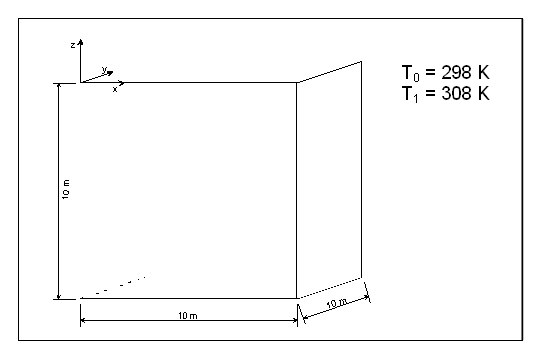
\includegraphics[width=0.6\textwidth]{TM/figures/fig61.eps}
\caption{Calculation area with one material}
\label{fig61}
\end{figure}

%\newpage

\textsl{Assumptions}

\begin{tabbing}
\=xxxxxxxxxxxx  \=xxxxxxxxxxxxxxxxxxxxxxx \kill
\> Temperature: \> constant temperature in the whole body at the beginning, heating \\
\> \> of the body about 10~K \\[1.0ex]
\> Solid: \> homogeneous, anisotropic, finite dimensions, no deformation at the \\
\> \> boundaries, linear elastic material behaviour, isotropic thermal ex- \\
\> \> pansion, different thermal expansion for the materials
\end{tabbing}

\subsubsection{Model set-up of the 3~D numerical model}

The dimensions of this 3~D-model are 10~m in all directions. Deformations perpendicular to the outer surfaces are suppressed. The initial temperature in the whole area is 298~K. At the top and at the bottom of the model thermal boundary conditions are set with a temperature of 308~K. Thereby the heating of the solid about 10~K is simulated. The used parameters of the solid represent the material behaviour of concrete (Tab. \ref{tab61}). 1000 elements and 1331 nodes are used. The calculation is divided in 384 time steps with a constant time step length of 900 seconds. That means the heating of the solid within 4 days is simulated. The calculation model is sketched in Fig. \ref{fig62}.
\begin{table}[htbp]
\centering
\begin{tabular}{|c|l|l|}
\hline
symbol & quantity & value \\
\hline
$T_0$  & Initial temperature (before heating) & 298 K \\
\hline
$T_1$  & Temperature after heating & 308 K \\
\hline
$\rho$  & Density of the solid &  2.2 t$\cdot$m$^{-3}$  \\			
\hline
$E$ & Young's modulus of the solid & 25 GPa \\
\hline
$\nu$ & Poisson ratio & 0.27 \\
\hline
$\alpha$ & Thermal expansion & 6.0$\cdot$10$^{-6}$ K$^{-1}$ \\
\hline
$c$      & Thermal capacity & 1.0 J$\cdot$kg$^{-1}\cdot$K$^{-1}$ \\
\hline
$\kappa$ & Thermal conductivity & 1.0 W$\cdot$m$^{-1}\cdot$K$^{-1}$ \\
\hline
\end{tabular}
\caption{Used parameters}
\label{tab61}
\end{table}

\begin{figure}[htbp]
\centering
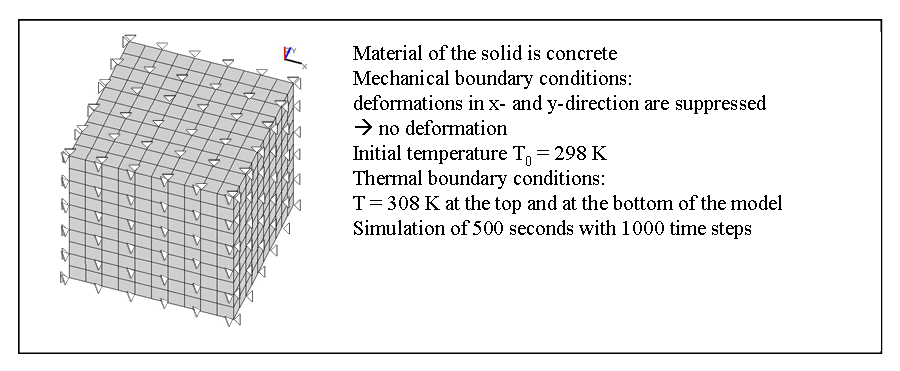
\includegraphics[width=0.9\textwidth]{TM/figures/fig62.eps}
\caption{Calculation model (3~D)}
\label{fig62}
\end{figure}

%\newpage

\subsubsection{Evaluation method}

The analytical solution can be derived from the time independent Eqns. \ref{eq61} to \ref{eq63} with the assumptions of no deformation and an isotropic thermal expansion:
\begin{eqnarray}
\varepsilon_i & \equiv & 0 \nonumber \\[1.5ex]
\sigma_x & = & \sigma_y\,=\,\sigma_z\,=\,
-\frac{\alpha\cdot\Delta T\cdot E}{1-2\cdot\nu}
\label{eq64}
\end{eqnarray}
Eqn. \ref{eq64} provides the stresses after heating the solid and shows an isotropic state of stress.

\subsubsection{Results}

With the analytical solution in Eqn. \ref{eq64} and the used parameters the stress values in the solid amount. This isotropic state of stress is reached after the whole solid is heated. The temporal development of the stresses in the centre of the model (at node 665) calculated is presented in Fig. \ref{fig63}. The results of the 3~D simulation show an exact agreement with the analytical solutions.

\begin{figure}[htbp]
\centering
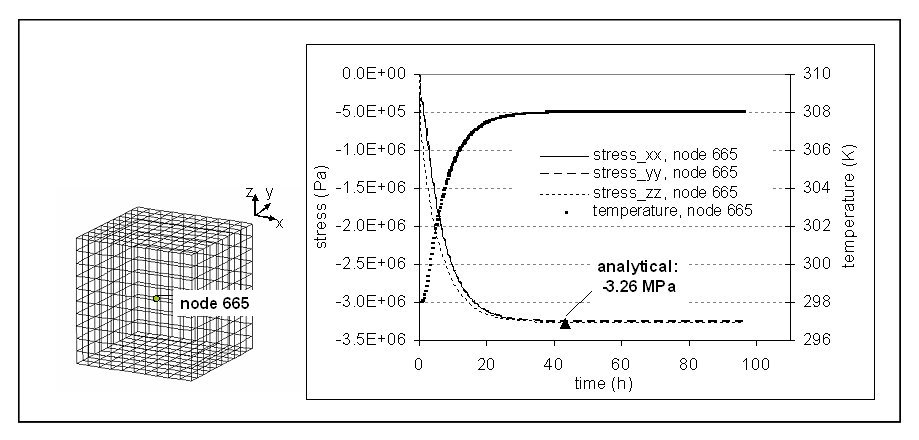
\includegraphics[width=0.9\textwidth]{TM/figures/fig63.eps}
\caption{Temporal stress development in the centre of the calculation model (node 665)}
\label{fig63}
\end{figure}

\begin{tabular}{|l|l|l|l|}
\hline
Path in the & Used code	& Used version & Date of simu- \\
benchmark deposit	& & & lation run \\
\hline	
TM$\backslash$heating$\backslash$cube$\backslash$	& GeoSys/RockFlow	& RockFlow 4,	rf4 & Dec. 2007 \\
tm\_01\_3Du	& & 4.05.07 & \\
\hline	
\end{tabular}


\subsection{Composite materials (3~D)}

\input{TM/ex6.1.2}

\subsection{Temperature increase in a hollow cylinder}


\subsubsection{Problem definition}

A hollow cylinder which consists of a solid of a constant temperature is exposed to a higher temperature at the surface of its hole. As a result of the increased temperature the cylinder is expanding. The aim of this calculation is to get out the radial displacement as well as the temperature distribution that are caused by the thermal expansion process by the use of an axisymmetric model. Fig. \ref{fig68} shows a sketch of the calculation area.

\begin{figure}[htbp]
\centering
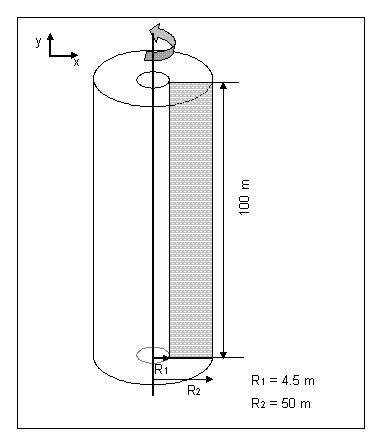
\includegraphics[width=0.45\textwidth]{TM/figures/fig68.eps}
\caption{Calculation area (grey area)}
\label{fig68}
\end{figure}


\textsl{Assumptions}

\begin{tabbing}
\=xxxxxxxxxxxx  \=xxxxxxxxxxxxxxxxxxxxxxx \kill
\> Temperature: \> constant temperature in the whole body at the beginning, heating \\
\> \> of the cylinder at the inner surface \\[1.0ex]
\> Solid: \> homogeneous, finite dimensions, no deformation in $y$-direction at \\
\> \> the bottom and the top, no deformation in $x$-direction at the right \\
\> \> border, linear elastic material behaviour, isotropic thermal expansion
\end{tabbing}

\subsubsection{Model set-up of the 2~D numerical model}

The axisymmetric model is in the $xy$-plane. The inner radius $R1$ of the cylindrical model is 4.5~m and the outer radius $R2$ 50~m. The cylinder is 100~m high. The initial temperature in the whole area is 25$^{\circ}$C. As boundary condition deformations in $y$-direction at the bottom and the top are suppressed, as well as deformations in $x$-direction at the right border. At the right boundary of the model a thermal boundary condition is set with a constant value of 25$^{\circ}$C. At the left boundary a source term for heat flux of $q=30$~W/m$^2$ is defined. Thereby the continuous heating of the solid is simulated. The used parameters of the solid are listed in Tab. \ref{tab63}. The simulation of only one time step is done. The numerical model consists of 766 elements and 426 nodes. It is sketched in Fig. \ref{fig69}.
\begin{table}[htbp]
\centering
\begin{tabular}{|c|l|l|}
\hline
symbol & quantity & value \\
\hline
$T_0$  & Initial temperature (before heating) & 25$^{\circ}$C \\
\hline
$q$  & Heat source & 30 W/m$^2$ \\
\hline
$\rho$  & Density of the solid &  2.0 t$\cdot$m$^{-3}$  \\			
\hline
$E$ & Young's modulus of the solid & 2.5 GPa \\
\hline
$\nu$ & Poisson ratio & 0.25 \\
\hline
$\alpha$ & Thermal expansion & 4.2$\cdot$10$^{-5}$ K$^{-1}$ \\
\hline
$\kappa$ & Thermal conductivity & 5.5 W$\cdot$m$^{-1}\cdot$K$^{-1}$ \\
\hline
\end{tabular}
\caption{Used parameters}
\label{tab63}
\end{table}

\begin{figure}[htbp]
\centering
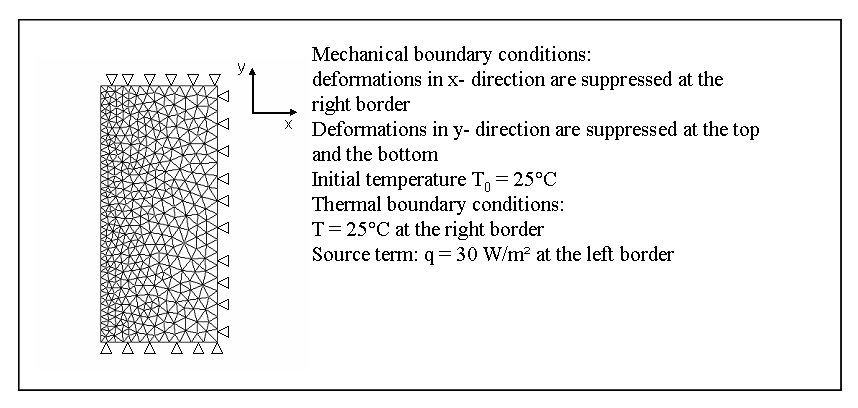
\includegraphics[width=0.9\textwidth]{TM/figures/fig69.eps}
\caption{Calculation model (2~D, axisymmetric) of the hollow cylinder}
\label{fig69}
\end{figure}

%\newpage

\subsubsection{Evaluation method}

For the hollow cylinder with the inner radius $R1$ and the outer radius $R2$ the following analytical solution for radial displacement $u_r$, stress $\sigma_r$ and temperature in dependency on the radius was used (Wang II, 2007).
\begin{eqnarray}
u_r & = &
\frac{q\,R_1\,\beta}{2\,\psi\,\kappa}\cdot r\cdot
\left(\ln\,r-\frac{1}{2}\right)\,+\,
\frac{A_0}{2}\,r\,+\,
\frac{A_1}{r}
\label{eq610} \\[2.0ex]
\sigma_r & = &
\psi\left[
-\frac{q\,R_1\,\beta}{2\,\psi\,\kappa}\cdot r\cdot
\left(\ln\,r+\frac{1}{2}\right)\,+\,
\frac{A_0}{2}\,-\,
\frac{A_1}{r^2}
\right] \nonumber \\[1.5ex]
 & & +\,
\lambda\left[
-\frac{q\,R_1\,\beta}{2\,\psi\,\kappa}\cdot r\cdot
\left(\ln\,r-\frac{1}{2}\right)\,+\,
\frac{A_0}{2}\,+\,
\frac{A_1}{r^2}
\right] \nonumber \\[1.5ex]
& & -\,\beta\left[
\frac{R_1\,q}{\kappa}\,\ln\left(\frac{R_2}{r}\right)\,+\,T_0
\right]
\label{eq611} \\[2.0ex]
T(r) & = &
\frac{R_1\,q}{\kappa}\,\ln\left(\frac{R_2}{r}\right)\,+\,T_0
\label{eq612}
\end{eqnarray}
{\small
where
\begin{displaymath}
\psi\,=\,\lambda\,+\,2\,G\qquad\mathrm{and}\qquad
\beta\,=\,\alpha\left(3\,\lambda\,+\,2\,G\right)
\end{displaymath}
with
\begin{tabbing}
\=xxxxxx \=xxxxxxxxxxxxxxxxxxxxxxxxxxxxxxxxx  \kill
\> $\lambda$   \> -- Lam$\acute{\mathrm{e}}$ elastic constant \\[0.5ex]
\> $G$         \> -- shear modulus \\[0.5ex]
\> $\alpha$    \> -- thermal expansion coefficient \\[0.5ex]
\> $\kappa$    \> -- thermal conductivity \\[0.5ex]
\> $A_0,\,A_1$ \> -- integration constants
\end{tabbing}
}

At the outer surface of the hollow cylinder (where $r=R_2$) there is no deformation, that means the displacement $u_{R2}$ is zero. Therefore Eqn. \ref{eq610} is set equal to zero for this boundary and adapted to $A_0$.
\begin{equation}
A_0\,=\,-\frac{2\,A_1}{R^2_2}\,-\,2\cdot B\cdot
\left(\ln\,R_2\,-\,\frac{1}{2}\right)
\label{eq613}
\end{equation}
{\small
where
}
\begin{displaymath}
B\,=\,\frac{q\,R_1\,\beta}{2\,\psi\,\kappa}
\end{displaymath}

At the inner surface of the hollow cylinder (where $r=R_1$) no stress is effected by the expansion because this boundary is phreatic. Therefore Eqn. \ref{eq611} is set equal to zero and $A_1$ is calculated by using Eqn. \ref{eq614}.
{\small
\begin{equation}
A_1=
\frac{
 \beta\!\left(\frac{
 \textstyle{R_1\,q}}{\textstyle{\kappa}}
 \ln\!\left(\frac{\textstyle{R_2}}{\textstyle{r}}\right)+T_0\right)
 \!+\!
 \lambda B\!\left(\ln R_1\!-\!\frac{1}{2}\right)\!+\!
 \psi B\!\left(\ln R_1\!+\!\frac{1}{2}\right)\!-\!
 \left(\frac{\textstyle{\lambda\!+\!\psi}}{\textstyle{2}}\right)
 2B\left(\ln R_2\!-\!\frac{1}{2}\right)
}
{\frac{
 \textstyle{\lambda-\psi}}{\textstyle{R^2_1}}-
 \frac{\textstyle{\lambda+\psi}}{\textstyle{2}}\cdot
 \frac{\textstyle{2}}{\textstyle{R^2_1}}\cdot
}
\label{eq614}
\end{equation}
}
After having solved this equation, $A_1$ is used to calculate $A_0$.
The results are:
\begin{eqnarray*}
A_0 & = & \phantom{-}5.96\cdot10^{-3} \\[1.0ex]
A_1 & = & -1.19\cdot10^{-1}
\end{eqnarray*}

\subsubsection{Results}

The results of the analytical equations for stresses, displacements and temperatures are compared to those of the numerical simulation by GeoSys/RockFlow. Fig. \ref{fig610} shows the temperature distribution over the radius of the hollow cylinder. In Fig. \ref{fig611} displacements in radial direction that are caused by the thermal expansion are depicted. In addition you can find the induced stresses in Fig. \ref{fig612}. Obviously, with the axisymmetric model a GeoSys/RockFlow simulation generates comprehensible results that meet well the analytic solution.

\begin{figure}[htbp]
\centering
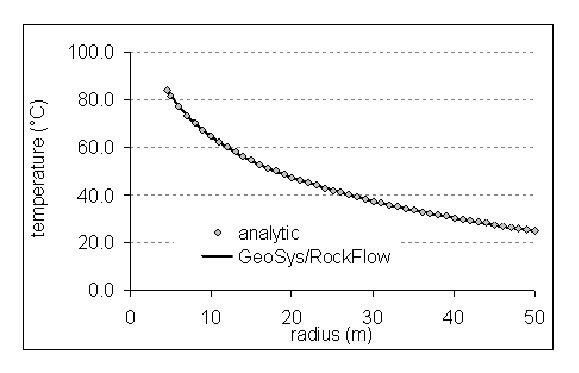
\includegraphics[width=0.75\textwidth]{TM/figures/fig610.eps}
\caption{Temperature distribution over the radius}
\label{fig610}
\end{figure}

\begin{figure}[htbp]
\centering
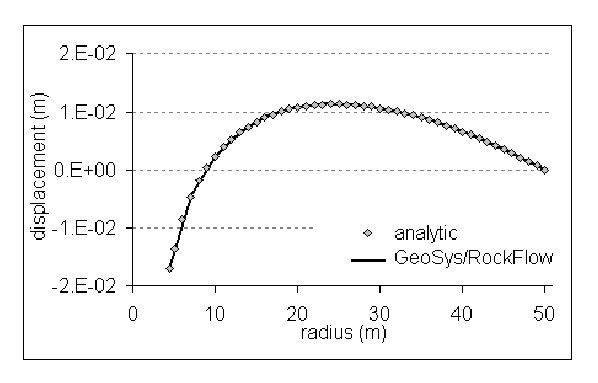
\includegraphics[width=0.75\textwidth]{TM/figures/fig611.eps}
\caption{Displacements in radial direction}
\label{fig611}
\end{figure}

\begin{figure}[htbp]
\centering
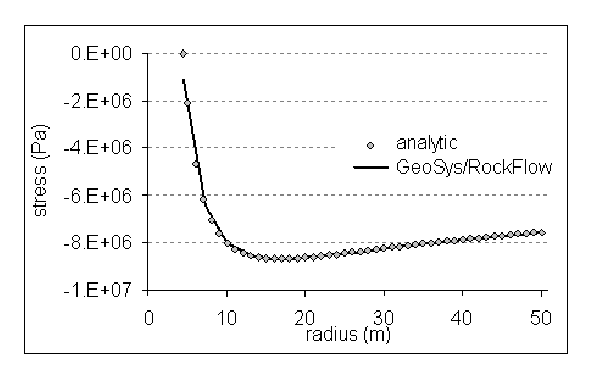
\includegraphics[width=0.75\textwidth]{TM/figures/fig612.eps}
\caption{Stresses in radial direction}
\label{fig612}
\end{figure}

\begin{tabular}{|l|l|l|l|}
\hline
Path in the & Used code	& Used version & Date of simu- \\
benchmark deposit	& & & lation run \\
\hline
$\backslash$TM$\backslash$heating$\backslash$hollowcylinder$\backslash$	& GeoSys/RockFlow	& RockFlow 4, & July 2007 \\
TM\_axi	& & rf4-502.exe & \\
\hline	
\end{tabular}

